\subsection{Caso de uso 2: Registrarse} \label{cu2}
\subsubsection{Resumen}
Este caso de uso le permite al usuario registrarse en el sistema proporcionando los datos solicitados.
\subsubsection{Descripción}
\begingroup
\setlength{\LTleft}{-10cm plus -1fill}
\setlength{\LTright}{\LTleft}
\begin{center}
  \addtocounter{table}{-1}
  \captionof{table}{Caso de uso 2: Registrarse} \label{tab:cu2_tab}
  \begin{longtable}{| p{3.5cm} | p{11.5cm} |}
      	\hline
      		\textbf{Versión} &  0.1 \\
        \hline 
       		\textbf{Autor} & Juan Gerardo Diaz Rodarte\\
        \hline
          \textbf{Estatus} & Edición \\
        \hline  
          \textbf{Fecha de último estatus} &  3 de abril de 2017 \\
        \hline
      \multicolumn{2}{|c|}{\large{Atributos}} \\
        \hline
          \textbf{Actor} & Usuario. \\
        \hline	
          \textbf{Disparador} & El actor abre la aplicación y presiona el botón de ¿Eres nuevo aquí?. \\
        \hline
          \textbf{Disparador} & El actor se registro exitosamente y es redirecionado. \\
        \hline
          \textbf{Entradas} & 
            \begin{itemize}
              \item \textbf{Correo electrónico}: Se escribe con el teclado.
              \item \textbf{Contraseña}: Se escribe con el teclado.
              \item \textbf{Confirmar contraseña}: Se escribe con el teclado.
              \item \textbf{Nombre(s)}: Se escribe con el teclado.
              \item \textbf{Apellido Paterno}: Se escribe con el teclado.
              \item \textbf{Apellido Materno}: Se escribe con el teclado.
              \item \textbf{Telefóno}: Se ingresa el código de país con un selector y el número con el teclado.
              \item \textbf{Fecha de nacimiento}: Se selecciona el año, mes y día con un selector.
              \item \textbf{Clave serial de dispositivo}: Se escribe con el teclado.
              \item \textbf{Vehículo}: Se selecciona de un selector.
            \end{itemize} \\
        \hline	
          \textbf{Salidas} &  
          \begin{itemize}
              \item \textbf{Interna}: Se mostrará el mensaje \textbf{\ref{msjn_04}} que indica que el registro fue exitoso.
            \end{itemize} \\
        \hline	
          \textbf{Precondiciones}& 
            \begin{itemize}
              \item \textbf{Interna:} El usuario debe de llenar todos los campos requeridos según la RNO.
            \end{itemize} \\
        \hline	
          \textbf{Postcondiciones} & 
            \begin{itemize}
              \item \textbf{Interna:} Al usuario se le generará una cuenta que necesita ser confirmada.
            \end{itemize} \\
        \hline    
           \textbf{Reglas de negocio} & 
             \begin{itemize}
               \item \textbf{\ref{rnl_01}}
               \item \textbf{\ref{rnl_02}}
               \item \textbf{\ref{rnl_03}}
               \item \textbf{\ref{rnl_04}}
               \item \textbf{\ref{rnl_05}}
               \item \textbf{\ref{rnl_06}}
               \item \textbf{\ref{rnl_09}}
               \item \textbf{\ref{rnrv_02}}
               \item \textbf{\ref{rnrv_03}}
               \item \textbf{\ref{rnrv_04}}
               \item \textbf{\ref{rnrv_05}}
               \item \textbf{\ref{rnrv_06}}
               \item \textbf{\ref{rnrv_07}}
               \item \textbf{\ref{rnrv_08}}
               \item \textbf{\ref{rnrv_11}}
               \item \textbf{\ref{rnrv_12}}
             \end{itemize} \\
        \hline
           \textbf{Mensajes} & 
              \begin{itemize}
                 \item \textbf{\ref{msja_01}}
                 \item \textbf{\ref{msje_02}}
                 \item \textbf{\ref{msje_03}}
                 \item \textbf{\ref{msje_04}}
                 \item \textbf{\ref{msje_05}}
                 \item \textbf{\ref{msje_06}}
                 \item \textbf{\ref{msje_07}}
                 \item \textbf{\ref{msje_08}}
                 \item \textbf{\ref{msjn_04}}
              \end{itemize}\\
        \hline
           \textbf{Tipo} & Primario \\
        \hline	    
  \end{longtable}
\end{center}
\endgroup

\subsubsection{Trayectorias del caso de uso}
\textbf{Trayectoria principal}
\begin{enumerate}
  \item {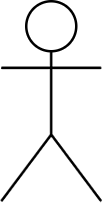
\includegraphics[scale=.1]{Capitulo3/img/actor.png} Ingresa el actor a la aplicación móvil, en el caso del administrador ingresa al portal web mediante una dirección eletrónica.}
  \item {
\includegraphics[scale=.05]{Capitulo3/img/proceso.png} Se muestar la vista IU Hogar. \hyperref[cu2_ta_a]{[Trayectoria alternativa A]}}
  \item {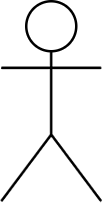
\includegraphics[scale=.1]{Capitulo3/img/actor.png} Selecciona el usuario la opción de \textit{¿Eres nuevo aquí?}}
  \item {
\includegraphics[scale=.05]{Capitulo3/img/proceso.png} Se muestar la vista IU Registro.}
  \item {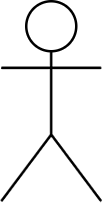
\includegraphics[scale=.1]{Capitulo3/img/actor.png} El actor ingresa los campos requeridos.}
  \item {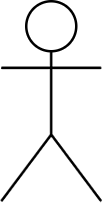
\includegraphics[scale=.1]{Capitulo3/img/actor.png} Presiona el botón para solicitar su registro al sistema.}
  \item {
\includegraphics[scale=.05]{Capitulo3/img/proceso.png} Verifica que el usuario haya ingresado la información requerida como establecido en la \textbf{\ref{rnl_01}}. \hyperref[cu2_ta_b]{[Trayectoria alternativa B]}}
  \item {
\includegraphics[scale=.05]{Capitulo3/img/proceso.png} Verifica que la dirección de correo electrónico cumpla con la \textbf{\ref{rnrv_02}}. \hyperref[cu2_ta_c]{[Trayectoria alternativa C]}}
  \item {
\includegraphics[scale=.05]{Capitulo3/img/proceso.png} Verifica que la contraseña cumpla con la \textbf{\ref{rnrv_03}}. \hyperref[cu2_ta_d]{[Trayectoria alternativa D]}}
  \item {
\includegraphics[scale=.05]{Capitulo3/img/proceso.png} Verifica que la contraseña de confirmación coincida con la contrasea ingresada. \hyperref[cu2_ta_e]{[Trayectoria alternativa E]}}
  \item {
\includegraphics[scale=.05]{Capitulo3/img/proceso.png} Verifica que el nombre cumpla con la \textbf{\ref{rnrv_04}}. \hyperref[cu2_ta_f]{[Trayectoria alternativa F]} \hyperref[cu2_ta_g]{[Trayectoria alternativa G]}}
  \item {
\includegraphics[scale=.05]{Capitulo3/img/proceso.png} Verifica que el apellido paterno cumpla con la \textbf{\ref{rnrv_04}}. \hyperref[cu2_ta_h]{[Trayectoria alternativa H]} \hyperref[cu2_ta_i]{[Trayectoria alternativa I]}}
  \item {
\includegraphics[scale=.05]{Capitulo3/img/proceso.png} Verifica que el apellido materno cumpla con la \textbf{\ref{rnrv_04}}. \hyperref[cu2_ta_h]{[Trayectoria alternativa H]} \hyperref[cu2_ta_i]{[Trayectoria alternativa I]}}
  \item {
\includegraphics[scale=.05]{Capitulo3/img/proceso.png} Verifica que el teléfono sea válido. \hyperref[cu2_ta_j]{[Trayectoria alternativa J]}}
  \item {
\includegraphics[scale=.05]{Capitulo3/img/proceso.png} Verifica que la fecha de nacimiento cumpla con la \textbf{\ref{rnrv_08}}. \hyperref[cu2_ta_k]{[Trayectoria alternativa K]}}
  \item {
\includegraphics[scale=.05]{Capitulo3/img/proceso.png} Verifica que la clave serial cumpla con la \textbf{\ref{rnrv_11}}. [\textbf{\ref{cu2_ta_l}}]}
  \item {
\includegraphics[scale=.05]{Capitulo3/img/proceso.png} Verifica que el vehículo seleccionado cumpla con la \textbf{\ref{rnrv_11}}. [\textbf{\ref{cu2_ta_m}}]}
  \item {
\includegraphics[scale=.05]{Capitulo3/img/proceso.png} Se muestra el mensaje \textbf{\ref{msjn_04}} que indica el registro exitoso al sistema.}
  \item {
\includegraphics[scale=.1]{Capitulo3/img/proceso.png} Se redirecciona a la vista IU Confirma tu teléfono.}\\
  \textit{Fin de caso de uso} \\	
\end{enumerate}

0\textbf{Trayectoria alternativa A} \phantomsection\label{cu2_ta_a} \\
\textbf{Condición:} El actor presiona la opción de \textit{Iniciar sesión}.\\
 \begin{enumerate}[label=A\arabic*]
  \item {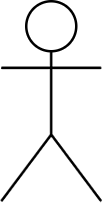
\includegraphics[scale=.1]{Capitulo3/img/actor.png} Presiona el botón de Iniciar sesión.}
  \item {
\includegraphics[scale=.05]{Capitulo3/img/proceso.png} Se muestar la vista IU Iniciar sesión.}
    \item {Continua en el paso 3 de la trayectoria principal.} \\
    \textit{Fin de trayectoria} \\
\end{enumerate}

\textbf{Trayectoria alternativa B} \phantomsection\label{cu2_ta_b} \\
\textbf{Condición:} El actor no proporcionó la información requerida, rompiendo la regla de negocio \textbf{\ref{rnl_01}}.\\
 \begin{enumerate}[label=B\arabic*]
    \item {
\includegraphics[scale=.05]{Capitulo3/img/proceso.png} Muestra el mensaje \textbf{\ref{msja_01}}, indicando que el actor ha dejado campos en blanco.}
    \item {Continua en el paso 5  de la trayectoria principal.} \\
    \textit{Fin de trayectoria} \\
\end{enumerate}

\textbf{Trayectoria alternativa C} \phantomsection\label{cu2_ta_c}\\
\textbf{Condición:} El actor no ingreso una dirección de correo electrónico que cumpla con la regla de negocio \textbf{\ref{rnrv_02}}.\\
 \begin{enumerate}[label=C\arabic*]
    \item {
\includegraphics[scale=.05]{Capitulo3/img/proceso.png} Muestra el mensaje \textbf{\ref{msje_02}}, indicando que la dirección de correo electrónico no es válida.}
    \item {Continua en el paso 5 de la trayectoria principal.} \\
    \textit{Fin de trayectoria} \\
\end{enumerate}

\textbf{Trayectoria alternativa D} \phantomsection\label{cu2_ta_d}\\
\textbf{Condición:} El actor ingreso una contraseña incorrecta que no cumple con la regla de negocio \textbf{\ref{rnrv_03}}.\\
 \begin{enumerate}[label=D\arabic*]
    \item {
\includegraphics[scale=.05]{Capitulo3/img/proceso.png} Muestra el mensaje \textbf{\ref{msje_01}}, indicando que el actor ha ingresado datos incorrectos.}
    \item {Continua en el paso 5 de la trayectoria principal.} \\
    \textit{Fin de trayectoria} \\
\end{enumerate}

\textbf{Trayectoria alternativa E} \phantomsection\label{cu2_ta_e}\\
\textbf{Condición:} El acto no ingreso la misma contraseña en los campo \textit{Contraseña} y \textit{Confirmar contraseña} coincidan.\\
 \begin{enumerate}[label=E\arabic*]
    \item {
\includegraphics[scale=.05]{Capitulo3/img/proceso.png} Muestra el mensaje \textbf{\ref{msje_04}}, indicando que las contraseñas no coinciden.}
    \item {Continua en el paso 5 de la trayectoria principal.} \\
    \textit{Fin de trayectoria} \\
\end{enumerate}

\textbf{Trayectoria alternativa F} \phantomsection\label{cu2_ta_f}\\
\textbf{Condición:} El actor no ingreso un nombre que cumpla con la longitud establecida en la \textbf{\ref{rnl_03}}.\\
 \begin{enumerate}[label=F\arabic*]
    \item {
\includegraphics[scale=.05]{Capitulo3/img/proceso.png} Muestra el mensaje \textbf{\ref{msje_05}}, indicando que el nombre sobrepasa la longitud máxima.}
    \item {Continua en el paso 5 de la trayectoria principal.} \\
    \textit{Fin de trayectoria} \\
\end{enumerate}

\textbf{Trayectoria alternativa G} \phantomsection\label{cu2_ta_g}\\
\textbf{Condición:} El actor ingreso un nombre que contiene símbolos o carácteres de tipo númericos.\\
 \begin{enumerate}[label=G\arabic*]
    \item {
\includegraphics[scale=.05]{Capitulo3/img/proceso.png} Muestra el mensaje \textbf{\ref{msje_06}}, indicando que el nombre contiene carácteres de tipo númerico o símbolos.}
    \item {Continua en el paso 5 de la trayectoria principal.} \\
    \textit{Fin de trayectoria} \\
\end{enumerate}

\textbf{Trayectoria alternativa H} \phantomsection\label{cu2_ta_h}\\
\textbf{Condición:} El actor no ingreso un apellido que cumpla con la longitud establecida en la \textbf{\ref{rnl_04}} .\\
 \begin{enumerate}[label=H\arabic*]
    \item {
\includegraphics[scale=.05]{Capitulo3/img/proceso.png} Muestra el mensaje \textbf{\ref{msje_05}}, indicando que alguno de los apellidos sobrepasa la longitud máxima.}
    \item {Continua en el paso 5 de la trayectoria principal.} \\
    \textit{Fin de trayectoria} \\
\end{enumerate}

\textbf{Trayectoria alternativa I} \phantomsection\label{cu2_ta_i}\\
\textbf{Condición:} El actor ingreso un apellido que contiene símbolos o carácteres de tipo númericos.\\
 \begin{enumerate}[label=I\arabic*]
    \item {
\includegraphics[scale=.05]{Capitulo3/img/proceso.png} Muestra el mensaje \hyperref[msje_06]{MSJE 06}, indicando que el apellido contiene carácteres de tipo númerico o símbolos.}
    \item {Continua en el paso 5 de la trayectoria principal.} \\
    \textit{Fin de trayectoria} \\
\end{enumerate}

\textbf{Trayectoria alternativa J} \phantomsection\label{cu2_ta_j}\\
\textbf{Condición:} El actor ingreso teléfono que no coincide con la longitud establecida en la \hyperref[rnrv_05]{RNRV 05} y \hyperref[rnrv_06]{RNRV 06} ó \hyperref[rnrv_07]{RNRV 07} .\\
 \begin{enumerate}[label=J\arabic*]
    \item {
\includegraphics[scale=.05]{Capitulo3/img/proceso.png} Muestra el mensaje \textbf{\ref{msje_07}}, indicando que la longitud del número celular es inválida.}
    \item {Continua en el paso 5 de la trayectoria principal.} \\
    \textit{Fin de trayectoria} \\
\end{enumerate}

\textbf{Trayectoria alternativa K} \phantomsection\label{cu2_ta_k}\\
\textbf{Condición:} El actor ingreso una fecha de nacimiento que no cumple con la \textbf{\ref{rnrv_08}}.\\
 \begin{enumerate}[label=K\arabic*]
    \item {
\includegraphics[scale=.05]{Capitulo3/img/proceso.png} Muestra el mensaje \textbf{\ref{msje_07}}, indicando que la longitud del número celular es inválida.}
    \item {Continua en el paso 5 de la trayectoria principal.} \\
    \textit{Fin de trayectoria} \\
\end{enumerate}

\textbf{\textlabel{Trayectoria alternativa L}{cu2_ta_l}}\\
\textbf{Condición:} El actor ingreso una clave serial que no cumple con la \textbf{\ref{rnrv_11}}.\\
 \begin{enumerate}[label=L\arabic*]
    \item {
\includegraphics[scale=.05]{Capitulo3/img/proceso.png} Muestra el mensaje \textbf{\ref{msje_12}}, indicando que la longitud del número celular es inválida.}
    \item {Continua en el paso 5 de la trayectoria principal.} \\
    \textit{Fin de trayectoria} \\
\end{enumerate}

\textbf{\textlabel{Trayectoria alternativa M}{cu2_ta_m}}\\
\textbf{Condición:} El actor selecciono un vehículo que no cumple con la \textbf{\ref{rnrv_12}}.\\
 \begin{enumerate}[label=M\arabic*]
    \item {
\includegraphics[scale=.05]{Capitulo3/img/proceso.png} Muestra el mensaje \textbf{\ref{msje_13}}, indicando que la longitud del número celular es inválida.}
    \item {Continua en el paso 5 de la trayectoria principal.} \\
    \textit{Fin de trayectoria} \\
\end{enumerate}

\textbf{\textlabel{Trayectoria alternativa N}{cu2_ta_n}}\\
\textbf{Condición:} El actor selecciono la opción de \textit{¿Has olvidado tu contraseña?}.\\
 \begin{enumerate}[label=N\arabic*]
    \item {
\includegraphics[scale=.05]{Capitulo3/img/proceso.png} Se ejecuta el \nameref{cu1_1}} \\
    \textit{Fin de trayectoria} \\
\end{enumerate}

\textbf{\textlabel{Trayectoria alternativa O}{cu2_ta_o}}\\
\textbf{Condición:} El actor selecciono la opción de \textit{¿Ya tienes una cuenta?}.\\
 \begin{enumerate}[label=O\arabic*]
    \item {
\includegraphics[scale=.05]{Capitulo3/img/proceso.png} Se ejecuta el \nameref{cu1}}\\
    \textit{Fin de trayectoria} \\
\end{enumerate}

\subsubsection{Puntos de extensión}
\noindent \textbf{Causa de la extensión:} El actor, de tipo de Usuario o Sub-Usuario, selecciono \textit{¿Has olvidado tu contraseña?} \\
\textbf{Región de la trayectoria:} \textbf{\ref{cu2_ta_n}} \\
\textbf{Extiende a:} \nameref{cu1_1} \\ \par

\noindent \textbf{Causa de la extensión:} El actor, de tipo de Usuario o Sub-Usuario, selecciono \textit{¿Ya tienes una cuenta?} \\
\textbf{Región de la trayectoria:} \textbf{\ref{cu2_ta_o}} \\
\textbf{Extiende a:} \nameref{cu1}
